%%%%%%%%%%%%%%%%%%%%%%%%%%%%%%%%%%%%%%%%%%%%%%%%%%%%%%%%%%%%%%%%%%%%%%%%
%
%
%     This file is included from the file   Segmentation.tex
% 
%     Section tag and label are placed in this top file.
%
%
%
%%%%%%%%%%%%%%%%%%%%%%%%%%%%%%%%%%%%%%%%%%%%%%%%%%%%%%%%%%%%%%%%%%%%%%%%



\itkpiccaption[Zero Set Concept]{Concept of Zero Set in a Level Set.\label{fig:LevelSetZeroSet}}
\parpic(9cm,6cm)[r]{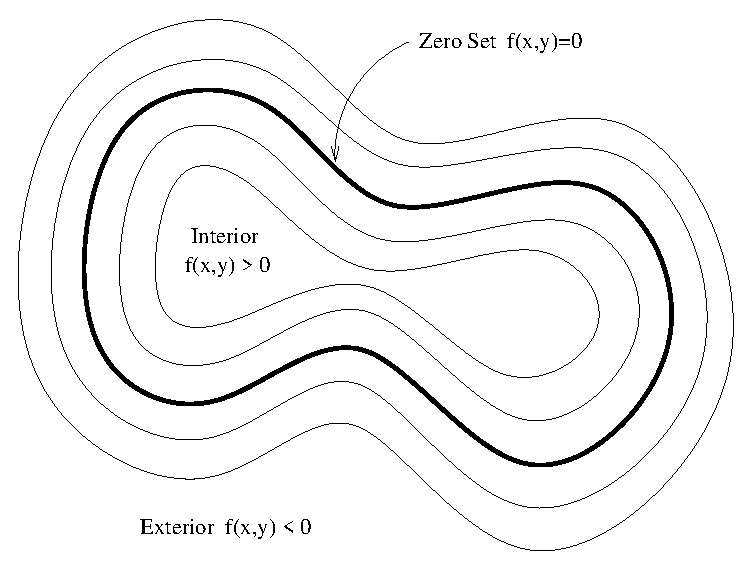
\includegraphics[width=8cm]{LevelSetZeroSet.eps}}

The paradigm of Level Set is a numerical method for tracking the evolution of
contours and surfaces. Instead of manipulating the contour directly, the
contour is embedded as the zero level set of a higher dimensional function
called the level-set function, $\psi(\bf{X},t)$. The level-set function is then
evolved under the control of a differential equation.  At any time, the evolving
contour can be obtained by extracting the zero level-set $\Gamma(\bf(X),t) =
\{\psi(\bf{X},t) = 0\}$ from the output.  The main advantages of using level
sets is that arbitrarily complex shapes can be modeled and topological
changes such as merging and splitting are handled implicitly. 

Level sets can be used for image segmentation by using image-based features such
as mean intensity, gradient and edges in the governering differential equation. 
In a typical approach, a contour is initialized by a user and is then evolved 
until it fits the form of an anatomical structure in the image. 
Many different implementations and variants of this basic concept have been
published in the literature. An overview of the field has been made by Sethian
\cite{Sethian1996}. 

The following sections introduce practical examples of some
of the Level Set segmentation methods available in ITK.  The remainder of this
section describes features common to all of these filters except the
\code{FastMarchingImageFilter}, which is derived from a different code
framework.  Understanding these features will aid in using the filters
more effectively.

Each filter makes use of a generic level-set equation to compute the update to
the solution $\psi$ of the partial differential equation.

\begin{equation}
\label{eqn:LevelSetEquation}
\frac{d}{dt}\psi = -\alpha \mathbf{A}(\mathbf{x})\cdot\nabla\psi - \beta
  P(\mathbf{x})\mid\nabla\psi\mid + \gamma Z(\mathbf{x})\kappa
\end{equation}
 
where $\mathbf{A}$ is an advection term, $P$ is a propagation (expansion) term,
and $Z$ is a spatial modifier term for the mean curvature $\kappa$.  The scalar
constants $\alpha$, $\beta$, and $\gamma$ weight the relative influence of
each of the terms on the movement of the interface.  A segmentation filter may
use all of these terms in its calculations, or it may omit one or more terms.
If a term is left out of the equation, then setting the corresponding scalar
constant weighting will have no effect.

All of the level-set based segmentation filters \emph{must} operate with
floating point precision to produce valid results.  The third, optional
template parameter is the \emph{numerical type} used for calculations and as
the output image pixel type.  The numerical type is \code{float} by default,
but can be changed to \code{double} for extra precision.  A user-defined,
signed floating point type that defines all of the necessary arithmetic
operators and has sufficient precision is also a valid choice.  You should not
use types such as \code{int} or \code{unsigned char} for the numerical
parameter.  If the input image pixel types do not match the numerical type,
those inputs will be cast to an image of appropriate type when the filter is
executed.

Most filters require two images as input, an initial model $\psi(\bf{X}, t=0)$,
and a \emph{feature image}, which is either the image you wish to segment or
some preprocessed version thereof.  You must specify the isovalue that
represents the surface $\Gamma$ in your initial model. The single image output of
each filter is the function $\psi$ at the final time step.  It is important to
note that the contour representing the surface $\Gamma$ is the zero level-set
of the output image, and not the isovalue you specified for the initial model.
To represent $\Gamma$ using the original isovalue, simply add that value back
to the output.

The solution $\Gamma$ is calculated to subpixel precision.  The best discrete
approximation of the surface is therefore the set of grid positions closest to
the zero-crossings in the image, as shown in
figure~\ref{fig:LevelSetSegmentationFigure1}.  The
\code{itk::ZeroCrossingImageFilter} operates by finding exactly those grid 
positions and can be used to extract the surface. 

\begin{figure}
\centering
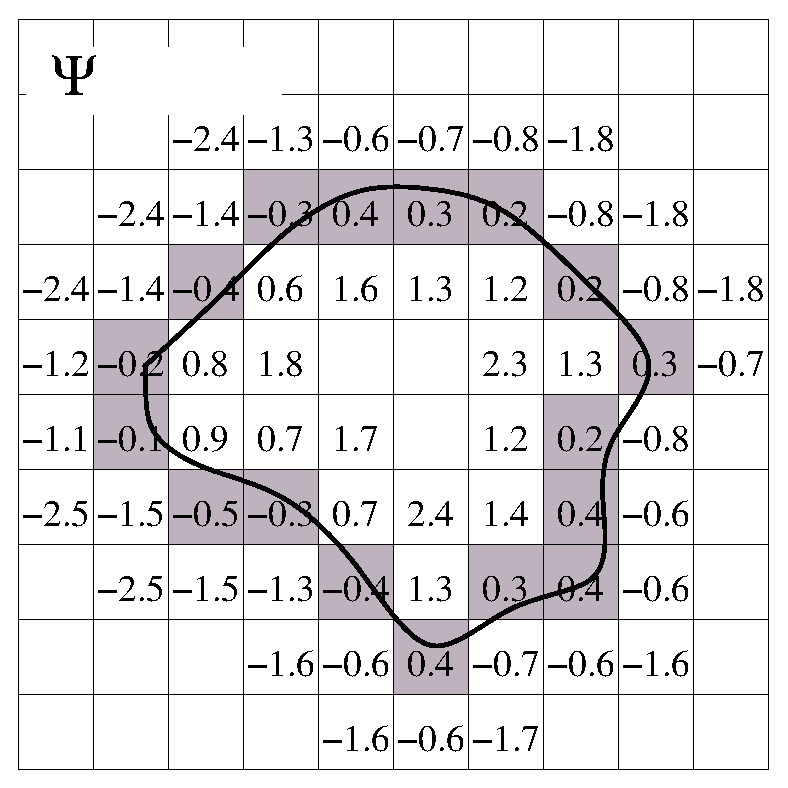
\includegraphics[width=0.4\textwidth]{LevelSetSegmentationFigure1.eps}
\itkcaption[Grid position of the embedded level-set surface.]{The implicit level
set surface $\Gamma$ is the black line superimposed over the image grid.  The location
of the surface is interpolated by the image pixel values.  The grid pixels
closest to the implicit surface are shown in gray. }
\protect\label{fig:LevelSetSegmentationFigure1}
\end{figure}

There are two important considerations when analyzing the processing time for
any particular level-set segmentation task: the surface area of the evolving
interface and the total distance that the surface must travel.  Because the
level-set equations are usually solved only at pixels near the surface (fast
marching methods are an exception), the time taken at each iteration depends on
the number of points on the surface.  This means that as the surface grows, the
solver will slow down proportionally.  Because the surface must evolve slowly
to prevent numerical instabilities in the solution, the distance the surface
must travel in the image dictates the total number of iterations required.

Some level-set techniques are relatively insensitive to initial conditions and are
therefore suitable for region-growing segmentation. Other techniques, like
\code{itk::LaplacianSegmentationLevelSetImageFilter}, can easily become
``stuck'' on image features close to their initialization and should be used
only when a reasonable prior segmentation is available as the initialization.
For best efficiency, your initial model of the surface should be the
best guess possible for the solution.  When extending the example applications
given here to higher dimensional images, for example, you can improve results
and dramatically decrease processing time by using a multi-scale
approach. Start with a downsampled volume and work back to the full resolution
using the results at each intermediate scale as the initialization for the next
scale.


\subsection{Fast Marching Segmentation}
\label{sec:FastMarchingImageFilter}

\ifitkFullVersion
\input{FastMarchingImageFilter.tex}
\fi



\subsection{Shape Detection Segmentation}
\label{sec:ShapeDetectionLevelSetFilter}

\ifitkFullVersion
\input{ShapeDetectionLevelSetFilter.tex}
\fi


\subsection{Geodesic Active Contours Segmentation}
\label{sec:GeodesicActiveContourImageFilter}

\ifitkFullVersion
\input{GeodesicActiveContourImageFilter.tex}
\fi


\subsection{Threshold Level Set Segmentation}
\label{sec:ThresholdSegmentationLevelSetImageFilter}
\ifitkFullVersion
\input{ThresholdSegmentationLevelSetImageFilter.tex}
\fi

\subsection{Canny-edge Level Set Segmentation}
\label{sec:CannySegmentationLevelSetImageFilter}
\ifitkFullVersion
\input{CannySegmentationLevelSetImageFilter.tex}
\fi

\subsection{Laplacian Level Set Segmentation}
\label{sec:LaplacianSegmentationLevelSetImageFilter}
\ifitkFullVersion
\input{LaplacianSegmentationLevelSetImageFilter.tex}
\fi


